
% Annual Cognitive Science Conference
% Sample LaTeX Paper -- Proceedings Format
% 

% Original : Ashwin Ram (ashwin@cc.gatech.edu)       04/01/1994
% Modified : Johanna Moore (jmoore@cs.pitt.edu)      03/17/1995
% Modified : David Noelle (noelle@ucsd.edu)          03/15/1996
% Modified : Pat Langley (langley@cs.stanford.edu)   01/26/1997
% Latex2e corrections by Ramin Charles Nakisa        01/28/1997 
% Modified : Tina Eliassi-Rad (eliassi@cs.wisc.edu)  01/31/1998
% Modified : Trisha Yannuzzi (trisha@ircs.upenn.edu) 12/28/1999 (in process)
% Modified : Mary Ellen Foster (M.E.Foster@ed.ac.uk) 12/11/2000
% Modified : Ken Forbus                              01/23/2004
% Modified : Eli M. Silk (esilk@pitt.edu)            05/24/2005
% Modified : Niels Taatgen (taatgen@cmu.edu)         10/24/2006
% Modified : David Noelle (dnoelle@ucmerced.edu)     11/19/2014
% Modified : Roger Levy (rplevy@mit.edu)     12/31/2018

%% Change "letterpaper" in the following line to "a4paper" if you must.

\documentclass[10pt,letterpaper]{article}

\usepackage{cogsci}
\usepackage{mathrsfs}  
\usepackage{graphicx}  
\usepackage{tipa}
\usepackage{booktabs}
\usepackage{tikz}
\cogscifinalcopy % Uncomment this line for the final submission 


\usepackage{pslatex}
\usepackage{apacite}
\usepackage{float} % Roger Levy added this and changed figure/table
                   % placement to [H] for conformity to Word template,
                   % though floating tables and figures to top is
                   % still generally recommended!

%\usepackage[none]{hyphenat} % Sometimes it can be useful to turn off
%hyphenation for purposes such as spell checking of the resulting
%PDF.  Uncomment this block to turn off hyphenation.
\usepackage{color}
\definecolor{Red}{RGB}{255,0,0}
\newcommand{\red}[1]{\textcolor{Red}{#1}}
\newcommand{\jd}[1]{\textcolor{Red}{[jd: #1]}}
\definecolor{Blue}{RGB}{0,100,255}
\newcommand{\blue}[1]{\textcolor{Blue}{#1}}
\newcommand{\lk}[1]{\textcolor{Blue}{[lk: #1]}}

%\setlength\titlebox{4.5cm}
% You can expand the titlebox if you need extra space
% to show all the authors. Please do not make the titlebox
% smaller than 4.5cm (the original size).
%%If you do, we reserve the right to require you to change it back in
%%the camera-ready version, which could interfere with the timely
%%appearance of your paper in the Proceedings.

\title{Probability and processing speed of scalar inferences is context-dependent}
 
% \author{{\large \textbf{Leyla Kursat}  {\normalfont and} \textbf{Judith Degen}}  \\
%  \{lkursat, jdegen\}@stanford.edu \\
%   Department of Linguistics, Stanford University \\
%   Stanford, CA 94305, USA}

\author{{\large \textbf{names}}  \\
 \{names\}@school\\
  Address}

\begin{document}

\maketitle

%\renewcommand{\citeA}{\textbf}
%\renewcommand{\cite}[1]{\textbf{(#1)}}

\begin{abstract}

 The past two decades have seen a wealth of studies addressing the question of whether or not scalar inferences -- whereby a listener takes a sentence like \textit{Alex ate some of the cookies} to mean that he did not eat all of them -- generally incur a processing cost, with conflicting results. This has spurred the development of studies seeking to understand the contextual conditions that facilitate scalar inferences. Here, we test a prediction made by \citeA{DegenTanenhaus2015}'s constraint-based account: that the probability of an interpretation and the speed with which it is processed is a function of the contextual support it receives. We manipulated the contextual support for the scalar inference in two truth-value judgment experiments  via the manipulation of a lexical feature (presence of partitive ``of the``) and a pragmatic feature (the implicit Question Under Discussion). Participants' responder type -- whether they generally produced pragmatic responses reflecting the inference or literal responses reflecting its absence -- was the main predictor of response times: pragmatic responses  were faster than literal responses when generated by a pragmatic responder, whereas the reverse was true for literal responders. This suggests that, rather than generally incurring a processing cost, inferences are easy to process by listeners who take the context to generally support the inference, and hard to process by listeners who take the context not to support the inference. We interpret this as evidence against literal-first or costly-implicature accounts and in support of constraint-based accounts of pragmatic processing.

\textbf{Keywords:} psycholinguistics; experimental pragmatics; scalar implicature; Question Under Discussion

\end{abstract}

\section{Introduction}

\jd{this is still the elm abstract -- need to flesh out each part in more detail}

The past two decades have seen a wealth of studies addressing the question of whether or not scalar inferences -- whereby a listener takes a sentence like \textit{Alex ate some of the cookies} to mean that he did not eat all of them -- generally incur a processing cost, with conflicting results \cite{BottNoveck2004,HuangSnedeker2009,Grodner2010,Breheny2013,DegenTanenhaus2016}. This has spurred the development of studies seeking to understand the contextual conditions that facilitate scalar inferences \cite{Zondervan2010,Degen2015,Augurzky2019,MartyChemla2013,DegenGoodman2014}.

Here, we test a prediction made by \citeA{DegenTanenhaus2015}'s constaint-based account: that the probability of an interpretation and the speed with which it is processed is a function of the contextual support it receives. In contrast, if scalar inferences generally incur a processing cost, pragmatic responses reflecting that the scalar inference was drawn should be slower to process than literal responses regardless of context. To test the constraint-based versus the costly inference account, we manipulated two features of context between participants in a truth-value judgement task: one lexical (\textit{presence of partititve "of"}) and one pragmatic (\textit{implicit QUD, see (1) and (2)}). This allowed us to obtain estimates of inference rate and processing speed. We further considered a participant’s \textit{responder type  --} whether they have a preference to respond literally or pragmatically -- as a predictive feature for response times. While the partitive and the QUD have previously been shown to affect the probability of drawing a scalar inference \cite{Zondervan2010,Degen2015,DegenGoodman2014,DegenTanenhaus2015}, contextual and participant-specific effects on processing speed have remained under-explored.

Implicit QUDs (manipulated via cover stories as in \citeA{Degen2013}):
\begin{enumerate}
  \item Did I get all of the gumballs? (\textit{all}-QUD, \textit{more supportive of scalar inference})
  \item Did I get any of the gumballs? (\textit{any}-QUD, \textit{less supportive of scalar inference})
\end{enumerate} 

\section{Experimental paradigm}

\begin{figure}
\fbox{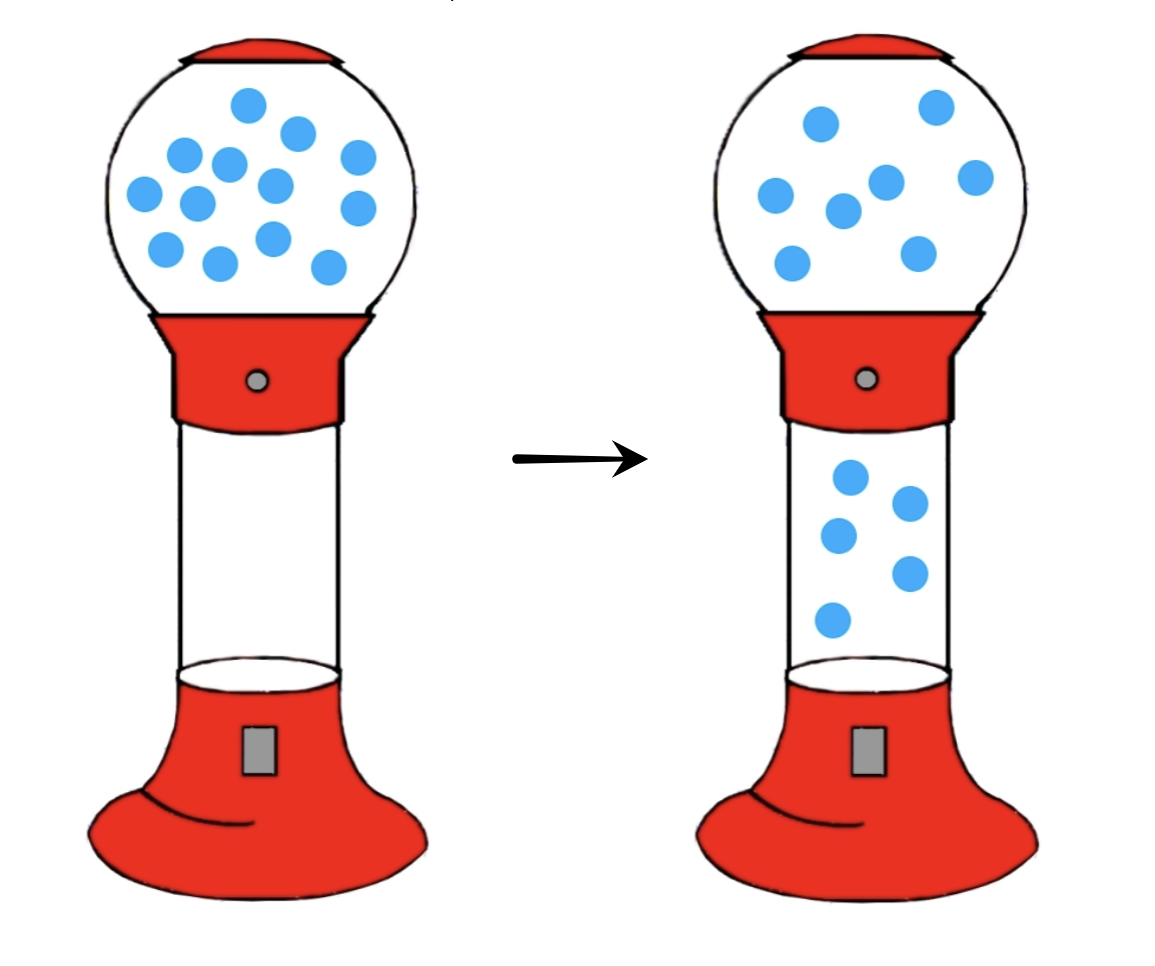
\includegraphics[width=\columnwidth]{./img/gumballs2.png}}
\caption{Example display from gumball paradigm. Left: initial display. Right: display with 5 gumballs dropped.  \label{fig:gumball-paradigm}}
\end{figure}

In both of our experiments, participants’ interpretations were probed using a ’gumball paradigm' introduced by \citeA{DegenTanenhaus2015}. On each trial, participants were shown a display of a gumball machine with 13 gumballs in the upper chamber and an empty lower chamber. After 4 seconds, some number of gumballs moved to the lower chamber and the machine reported how many gumballs were distributed (Fig.~\ref{fig:gumball-paradigm}). This pre-recorded statement was of the form "You got X gumballs", where X is a quantifier (\textit{some},  \textit{all}, \textit{none}, or a number between 1 and 13). The number of gumballs that are dropped to the lower chamber and the quantifier reported by the gumball machine were varied and they did not always match (see Table \ref{tab:stimuli}).

Participants were assigned to one of the two conditions (\textit{all}-QUD, \textit{any}-QUD) which differed in the cover story they were presented with at the beginning of the experiment. These cover stories were designed to establish an implicit QUD (see Table \ref{tab:coverstories}).

% \textbf{\textit{all}-QUD} Participants assigned to the \textit{all}-QUD condition read a cover story explaining that they are at a candy store helping the store worker test a row of special gumball machines. These gumball machines report how many gumballs they distribute but are sometimes incorrect in their report. Participants were also told that the store worker's boss has threatened to fire him if the gumaball machines are left empty and he cannot see the machines from the register and can only tell how full they are by their statements. Participants were asked to help the store worker by telling him if this statement is right or wrong by pressing the yes or no key. They were also told that they had 4 seconds to notify the store worker and they should make a decision as quickly as possible. 

% \begin{center}Is the machine empty? $\rightarrow$ Did I get all of the gumballs?\end{center}

% \textbf{\textit{any}-QUD} Participants in the \textit{any}-QUD condition read the same cover story except in their story, the gumball machines sometimes jam and don't deliver gumballs. The store worker's boss has threatened to fire him if the gumball machines stay jammed.

% \begin{center}Is the machine jammed? $\rightarrow$ Did I get any of the gumballs?\end{center}

  \begin{table}
      \begin{tabular}{lccccccc}
      \midrule
      \multicolumn{8}{c}{\textbf{Set size}} \\
      \textbf{Quantifier} & 0 & 2 & 5 & 8 & 11 & 13 & \multicolumn{1}{l}{\textbf{Total}} \\
      \midrule
      \textit{some/some of} & 4 & 1 & 1 & 1 & 1 & 8 & 16 \\
      \textit{all of} & 2 & 1 & 2 & 1 & 2 & 8 & 16 \\
      \textit{none of} & 4 & 1 & 0 & 1 & 1 & 1 & 8 \\
      number & 3 & 7 & 7 & 7 & 5 & 3 & 32 \\
      \bottomrule
      \textbf{Total} & 13 & 10 & 10 & 10 & 9 & 20 & 72
      \end{tabular}
    \caption{Distribution of experimental trials over quantifiers and set sizes.\label{tab:stimuli}}
  \end{table}

  \begin{table*}[]
    \begin{tabular}{cclll}
      \cline{1-2}
      \toprule
      \textbf{all-QUD} & \textbf{any-QUD} &  &  &  \\
      \midrule
      \multicolumn{2}{c}{\begin{tabular}[c]{@{}c@{}}You are at a candy store and are testing a row of gumball machines. These are special \\ gumball machines that say how many gumballs you got. However, this report is \\ sometimes faulty.\end{tabular}} &  &  &  \\
      \midrule
      \begin{tabular}[c]{@{}c@{}}The store worker tells you that his boss has threatened \\ to fire him if the gumball machines are left empty, and he \\ really needs this job. He cannot see the machines from \\ the register, but he can normally tell how full they \\ are by the machines' statements.\end{tabular} & \begin{tabular}[c]{@{}c@{}}The store worker tells you that machines sometimes \\ jam and don't deliver any gumballs. His boss has \\ threatened to fire him if the gumball machines stay \\ jammed, and he really needs this job. He cannot see \\ the machines from the register, but he can normally \\ tell if they are working by the machines' statements.\end{tabular} &  &  &  \\
      \midrule
      \multicolumn{2}{c}{He asks you to tell him if the statement is right or wrong, so that he will know if a machine is empty and needs to be refilled.} &  &  &  \\
      \multicolumn{2}{c}{After you hear the statement, you have 4 seconds to notify the store worker, so please make a decision as quickly as possible.} &  &  & \\
      \bottomrule
      \end{tabular}
      \caption{Cover stories for each QUD condition.\label{tab:coverstories}}

  \end{table*}

\section{Experiment 1: Partitive statement}

In experiment 1 we tested whether the QUD, as a contextual feature of an utterance, could modulate the probability of a scalar implicature and the speed with which it is processed. The main prediction was that in the \textit{all}-QUD condition, the implicit QUD "Did I get all of the gumballs", would be more relevant to the "You got all of the gumballs" interpretation. Thus, there would be more pragmatic "disagree" responses in the critical trials when participants hear "You got some of the gumballs" and get all 13 gumballs. We also predicted that the relevance of the QUD would increase the speed of pragmatic responses and slow down the literal responses.

Procedure, materials, analyses and exclusions were pre-registered on OSF and will be available upon publiciation along with data and experiment scripts.

\subsection{Methods}

\paragraph{Participants}
We recruited 800 participants on Amazon Mechanical Turk. Participants were required to have a US-based IP address and a minimal approval rating of 95\%. They were paid \$2.3.

\paragraph{Materials and procedure}
After reading the cover story of their QUD condition, participants went through a scripted demonstration that showed the consequences of store worker's responses to various scenarios. To ensure that they paid attention to the cover story, they were asked a multiple choice question about when the store worker will be fired. When participants answered this question incorrectly, they were presented with the cover story again and went through the same demonstration. Halfway through the experiment, participants were asked to answer this multiple-choice question again. This was done to prevent the decay of the implicit QUD over time.

There were 4 practice trials with \textit{all} and \textit{none}. On half of these trials, the statements were correct, and on the other half they were incorrect. After the practice trials, there were 72 experimental trials. On 32 of the trials, the expected answer was yes, and on 32 of the trials, the expected answer was no. The remaining 8 trials were occurances of the critical trial and the main focus of this experiment. On these trials, all 13 gumballs dropped to the lower chamber and participants heard the partitive statement "You got \textit{some of} the gumballs". When participants press YES to agree with this statement, they interpret it semantically as "You got some, and possibly all, of the gumballs" and when they press NO to disagree, they interpret it pramatically as "You got some, but not all, of the gumballs". 

\noindent \textbf{Exclusions} We excluded participants who were self-reported non-native English speakers (n=X), participants who got the second cover story comprehension questions wrong more than twice (n=Y) and participants with accuracy lower than 85\% on non-critical trials (n=Z). Only responses to critical trials are reported below.

\subsection{Results and discussion}

\noindent \textbf{Judgements}

Proportion of pragmatic responses on critical trials are shown in Figure~\ref{fig:judgements}. 78\% of responses given by the participants in the \textit{all}-QUD condition were pragmatic compared to 71\% pragmatic responses given by participants in the \textit{any}-QUD condition. We ran a mixed effects logistic regression predicting response type with random by-participant intercepts from fixed effects of QUD and found a main effect of QUD such that there are more pragmatic responses for \textit{all}-QUD compared to \textit{any}-QUD ($\beta$=1.31, SE=0.52, p$<$.05). In the \textit{all}-QUD condition, the cover story made the question participants were trying to answer more relevant to the "You got all of the gumballs" interpretation and participants were more likely to respond pragmatically.

\noindent \textbf{Analysis of Variability in Judgements} 

 In order to asses participants' response consistency, we \lk{plotted} the distribution of participants over number of pragmatic responses given on critical trials (see Figure~\ref{fig:proportion}).  While there were people who were completely consistent, there was also some variability. For the purpose of the subsequent response time analyses, we divided participants into two groups. Following the procedure in \citeA{Degen2015}, we categorized participants with more than 4 pragmatic responses as pragmatic responders (38\%) and participants with less than 4 pragmatic responses as literal responders (60\%). \lk{X} participants (\lk{X\%}) gave an equal number of pragmatic and literal responses and were excluded from this analysis.

\noindent \textbf{Response Times} 

There was an interaction between QUD and response ($\beta$=-0.12, SE=0.03, t=-3.70, p$<$.0001) such that pragmatic responses were faster under the \textit{all}-QUD than under the \textit{any}-QUD. This shows that the QUD, as a feature of the context, not only affects the robustness but also the speed of scalar inferences. 

\lk{connect these two paragraphs}
There was also  an interaction between responder type and response ($\beta$=-0.28, SE=3.34, t=-8.37, p$<$.0001). Pragmatic responses were faster than literal responses for pragmatic responders and literal responses were faster than pragmatic responses for literal responders.

\begin{figure}
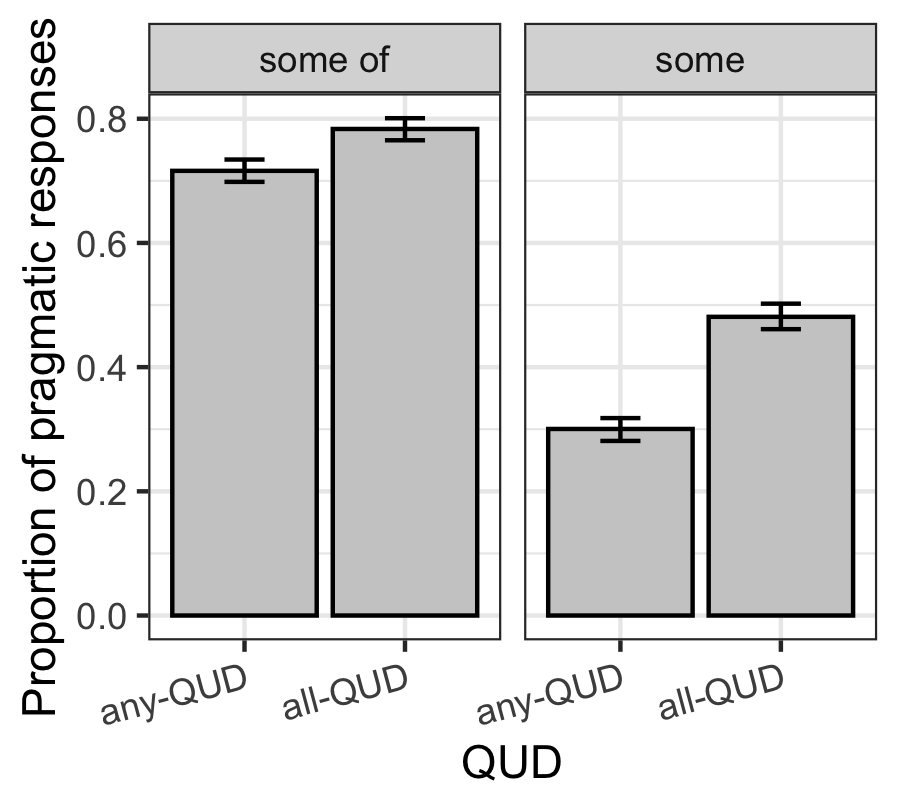
\includegraphics[width=\columnwidth]{plots/judgements.png}
\caption{Proportion of pragmatic responses on partitive "some of" (left) and non-partitive "some" (right) critical trials. Error bars indicate bootstrapped 95\% confidence intervals. \label{fig:judgements}}
\end{figure}

\begin{figure}
  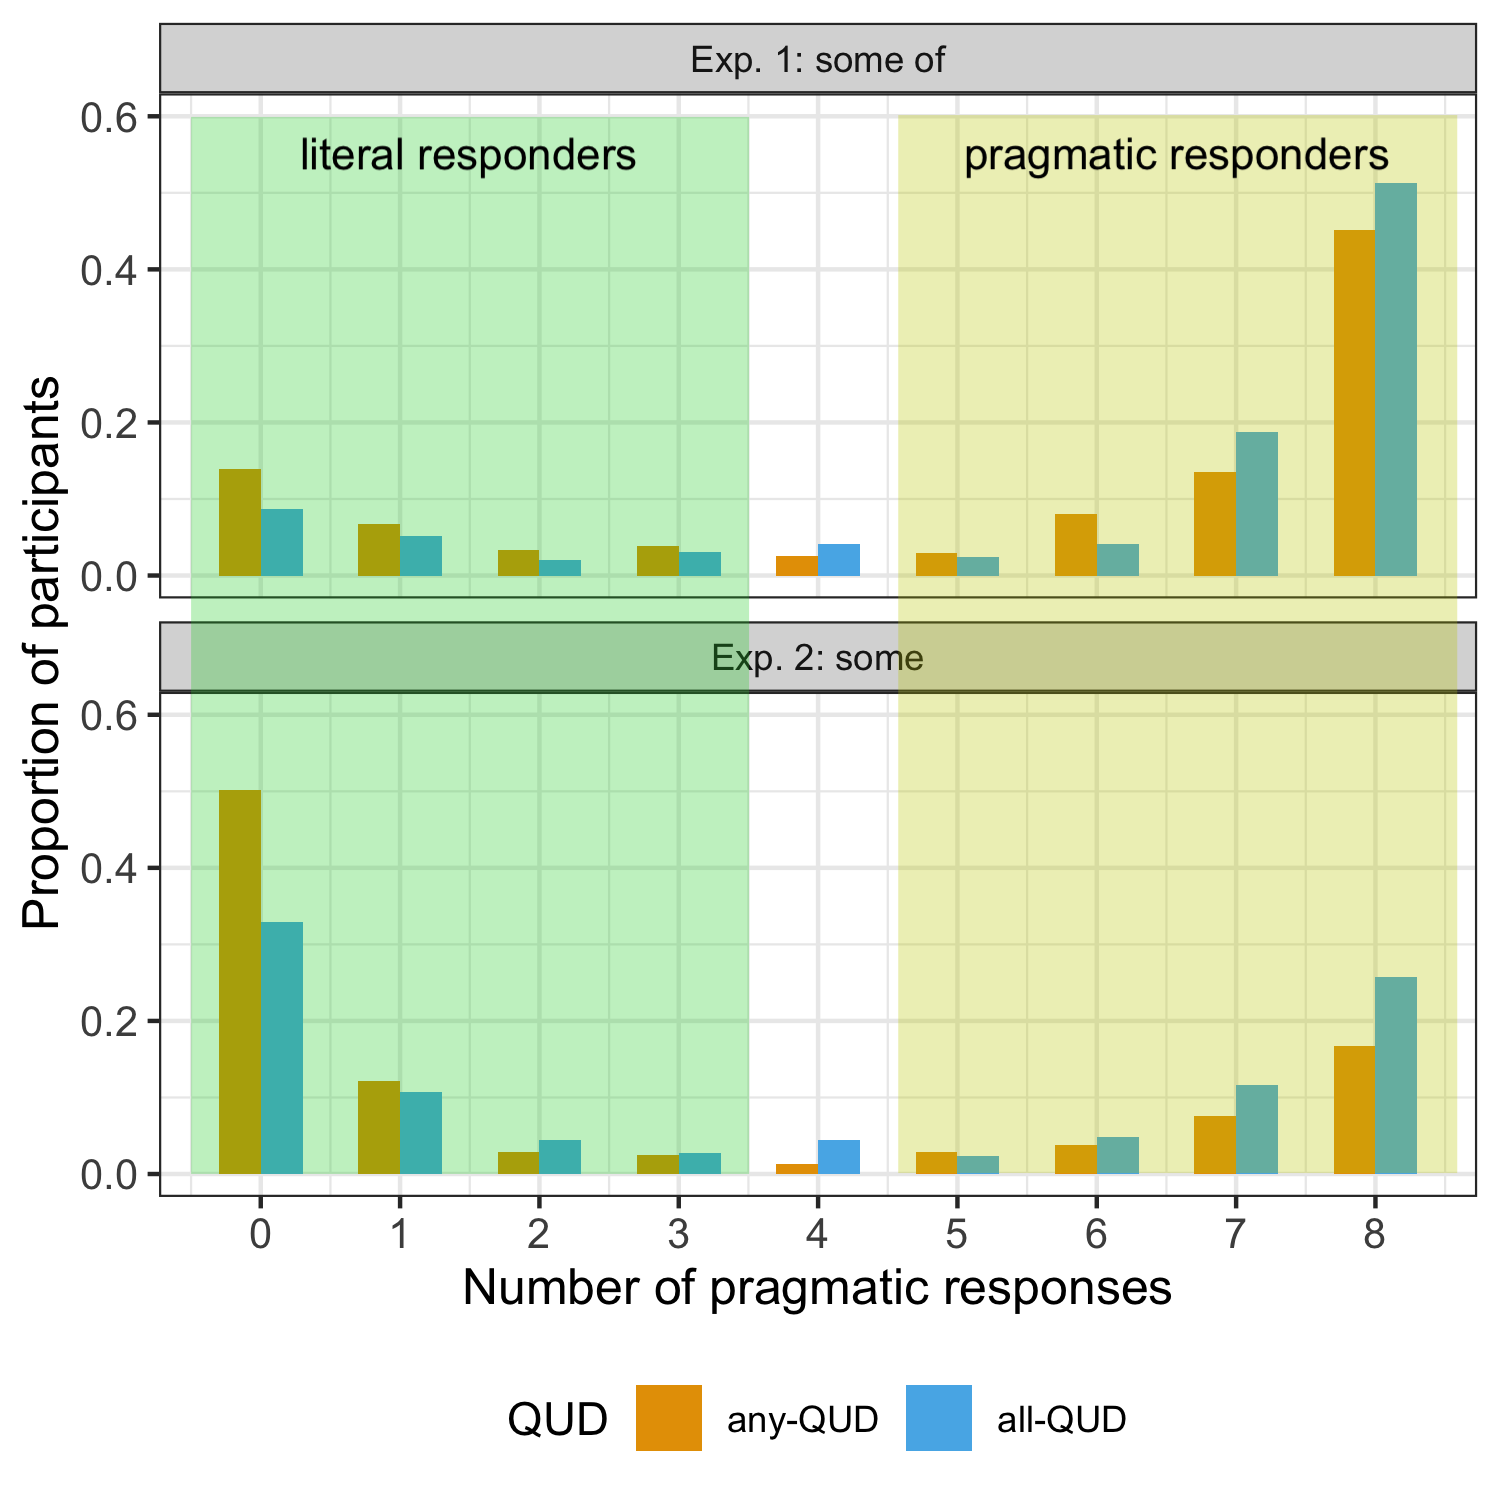
\includegraphics[width=\linewidth]{plots/proportion.png}
  \caption{Distribution of participants over number of pragmatic responses given on critical trials. \label{fig:proportion}}
\end{figure}

\section{Experiment 2: Non-partitive statement}

In Experiment 2 we tested whether the absence of the partitive, previously shown to decrease the contextual support for the inference, would decrease the inference strength and robustness of scalar implicatures,

% Experiment 2 was designed to test whether the contextual support provided by a lexical cue (absence of partitive "of") modulate robustness and speed of scalar inferences. Our main question was whether compared to Experiment 1 in which partitive "some" was used, would the lack of the partitive, previously shown to decrease inference strength, also slow down pragmatic responses and speed up literal responses compared to its partitive counterpart?

\subsection{Methods}

\noindent \textbf{Participants} We recruited 800 participants on Amazon Mechanical Turk. Participants were required to have a US-based IP address and a minimal approval rating of 95\%. They were paid \$2.3.

\noindent \textbf{Materials and procedure} The materials and procedures were the same as in Experiment 1 except on critical trials, when all 13 gumballs dropped to the lower chamber, participants heard the non-partitive statement "You got \textit{some} gumballs".

\noindent \textbf{Exclusions} As in Experiment 1, we excluded non-native English speakers (n=X), participants who got the second comprehension question wrong more than twice (n=Y), and participants that had accuracy lower than 85\% on non-critical trials (n=Z).

\subsection{Results and discussion}

\begin{figure}
  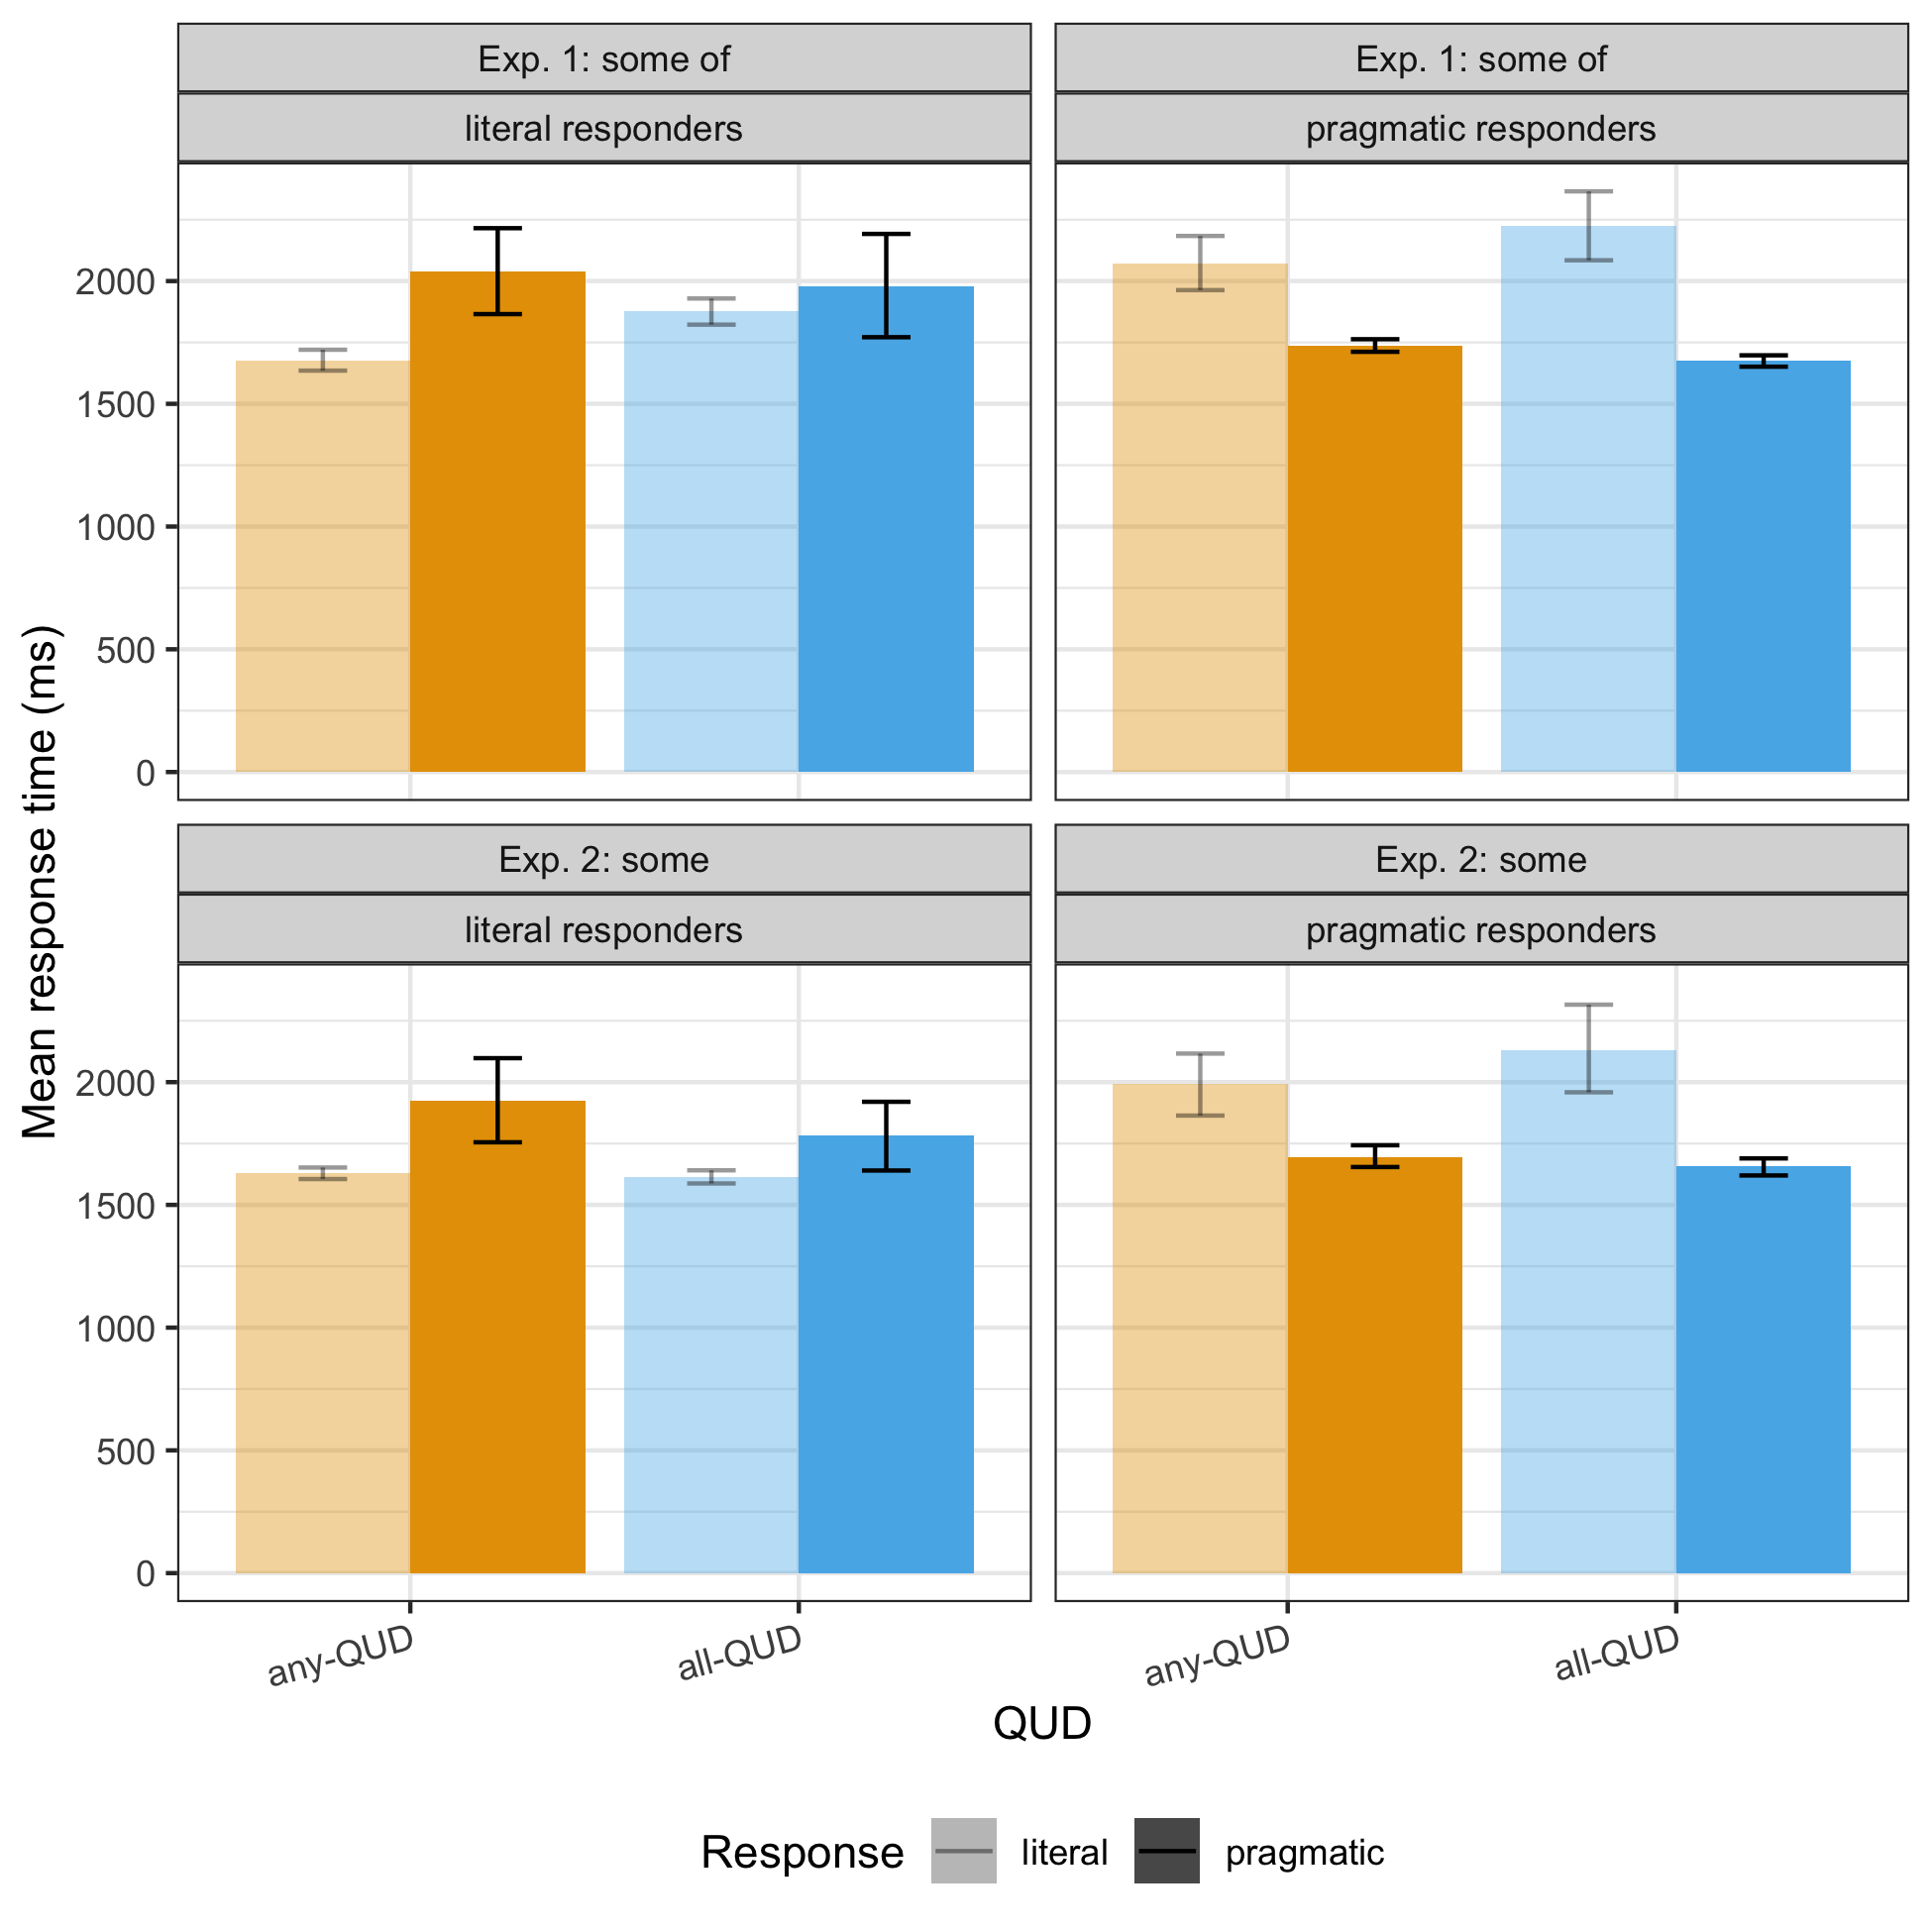
\includegraphics[width=\columnwidth]{plots/responsetimes.png}
  \caption{Mean response times for literal (green) and pragmatic (orange) responses generated by literal (upper panels) and pragmatic (lower panels) responders on partitive "some of" and non-partitive "some" critical trials. \label{fig:responsetimes}}
\end{figure}

\noindent \textbf{Judgements}

Replicating the QUD effect found in Experiment 1, we found that participants in the \textit{all}-QUD condition gave more pragmatic "disagree" responses than participants in the \textit{any}-QUD ($\beta$=4.69, SE=0.80, p$<$.0001). \lk{When data was pooled: pragmatic "disagree responses were more likely in the \textit{all}-QUD ($\beta$=2.85, SE=0.44, p$<$.0001) condition}

We found that overall, participants in Experiment 2 who heard the non-partitive statement were less likely to respond pragmatically compared to participants in Experiment 1 who heard its partitive countepart ($\beta$=7.16, SE=0.69, p$<$.0001)(see Fig~\ref{fig:judgements}).

We also found an interaction of the lexical cue and QUD ($\beta$=-3.06, SE=0.90, p$<$.0001) but it was due to the qud effect being bigger for the non-partitive condition than the partitive condition. \lk{This interaction is perhaps due to a ceiling effect.}

\noindent \textbf{Analysis of Variability in Judgements}

\lk{As shown in Figure~\ref{fig:proportion}, plot skewed..}

\noindent \textbf{Response Times}

When the non-partitive form was used, the QUD didn't affect the speed of scalar implicatures significantly, however when data was pooled from both experiments, there was a main effect of QUD such that \lk{fill}.

\lk{this analysis needs to be done separately for the two quantifiers because the stims differ in length?? - when done together: interaction of lexical cue and response ($\beta$=-4.07, SE=1.71, t=-2.38, p$<$.01)}

\lk{full model: interaction between qud and response ($\beta$=-1.07, SE=2.29, t=-4.67, p$<$.001), largest observed effect: interaction between responder type and response ($\beta$=-0.27, SE=0.02, t=-11.7, p$<$.0001), such that pragmatic responses were faster than literal responses for pragmatic responders and literal responses were faster than pragmatic responses for literal responders.}

\section{General discussion and conclusion}
\lk{from ELM abstract}

Overall, pragmatic "disagree" responses were more likely in the partitive ($\beta$=7.16, SE=0.69, p$<$.0001) and in the \textit{all}-QUD ($\beta$=2.85, SE=0.44, p$<$.0001) condition, replicating previous results.

This suggests that contextual factors affect listeners' overall contextual response strategy which in turn impacts the speed with which they process the preferred interpretation. This is evidence against costly inferece accounts and in support of constraint-based accounts.

\begin{figure}
  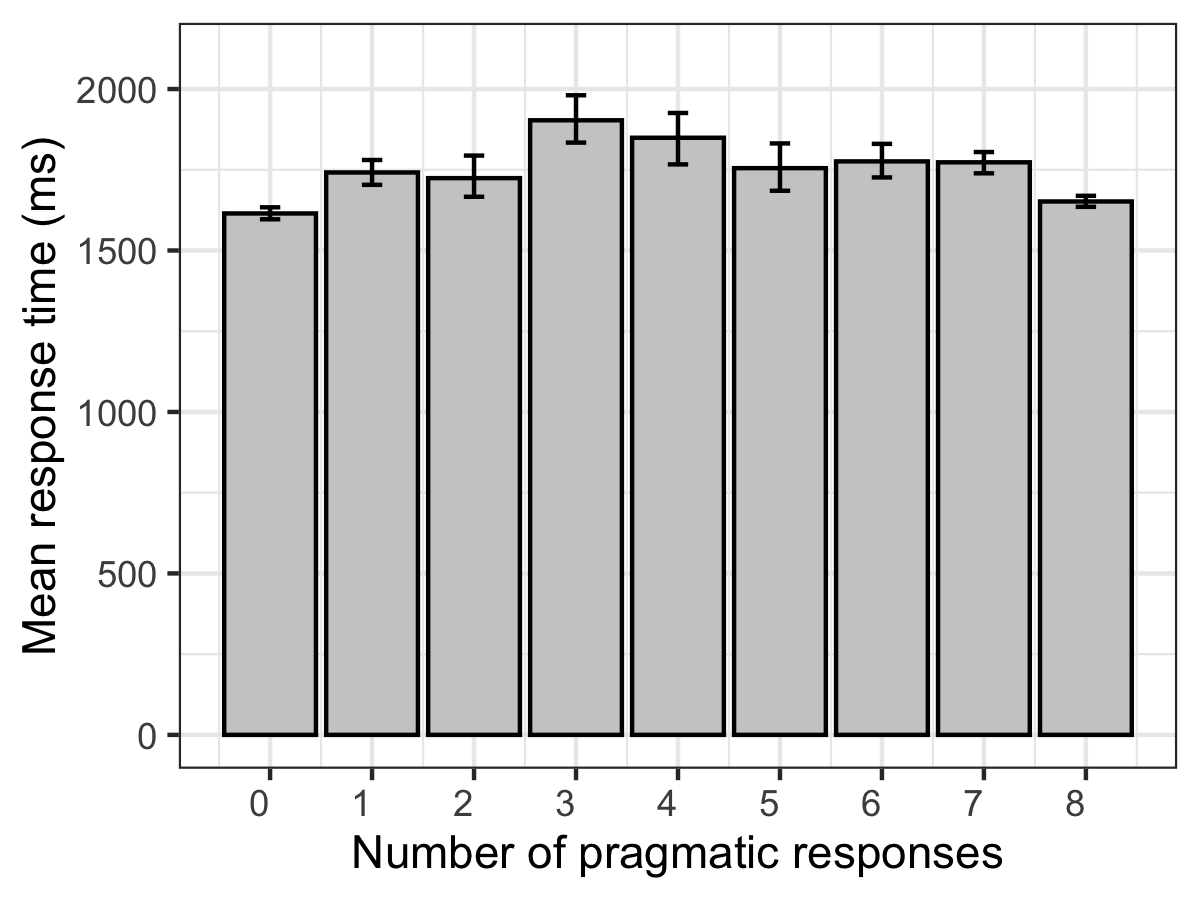
\includegraphics[width=\columnwidth]{plots/consistency.png}
  \caption{Mean response times for participants grouped based on the number of pragmatic responses they gave. \label{fig:consistency}}
\end{figure}

%\section{References Instructions}
%
%Follow the APA Publication Manual for citation format, both within the
%text and in the reference list, with the following exceptions: (a) do
%not cite the page numbers of any book, including chapters in edited
%volumes; (b) use the same format for unpublished references as for
%published ones. Alphabetize references by the surnames of the authors,
%with single author entries preceding multiple author entries. Order
%references by the same authors by the year of publication, with the
%earliest first.
%
%Use a first level section heading, ``{\bf References}'', as shown
%below. Use a hanging indent style, with the first line of the
%reference flush against the left margin and subsequent lines indented
%by 1/8~inch. Below are example references for a conference paper, book
%chapter, journal article, dissertation, book, technical report, and
%edited volume, respectively.


\bibliographystyle{apacite}

\setlength{\bibleftmargin}{.125in}
\setlength{\bibindent}{-\bibleftmargin}

\bibliography{cogsci}

\end{document}
